\documentclass[11pt]{article}
% Language setting
% Replace `english' with e.g. `spanish' to change the document language
\usepackage[english]{babel}
\usepackage{amssymb}
\usepackage{nccmath}
\usepackage{mathtools}
\usepackage{ragged2e}
% Set page size and margins
% Replace `letterpaper' with `a4paper' for UK/EU standard size
\usepackage[a4paper,top=2cm,bottom=2cm,left=3cm,right=3cm,marginparwidth=1.75cm]{geometry}
\usepackage{amsmath}
\usepackage{graphicx}
\usepackage[colorlinks=true, allcolors=blue]{hyperref}
\parindent 0pt
\title{IoT System for Forestry}
\begin{document}
\begin{titlepage}
    \centering
    \vspace*{\baselineskip}
    \centerline{
\includegraphics{logo uniurb.jpg}}
    \vskip 2.5 cm
    
    \Huge{\textbf{\scshape{IoT for the health of forests}}}
    \vskip 2.5 cm
    \large{\textbf{Bachelor's program in "IT: Science and Technology", University of Urbino}}

    \vskip 2.5 cm
    \centerline{\textbf{Project report for the exam of:}} 
    \centerline{\textbf{Systems for Internet of Things}} 
    \vskip 0.3cm
	\Large{\ Summer Session --- 2023/2024}
	
	    \vskip 2.0 cm
	
		{\large {\scshape student:}\\[0.3cm] Nicolas Barzotti\\ ID Number: 313687}\\ 
		[0.4cm]
        \vskip 2.5 cm
	     \large{{\scshape professor:} \\[0.3cm] Doc. Eng. Luca Romanelli}\\[1.3cm]		
    
    
\end{titlepage}
\raggedright

\begin{abstract}
\noindent As global warming takes its toll on the planet we must provide a solution just like we created the problem. IoT technology helps us with this through sensors and communication protocols that allow the least human interference possible in the natural world. To this effect the following paper proposes an experiment that uses a non intrusive sensory network capable of determining the possibility of forest fires sprouting and spreading in a forest environment. Such a project would allow for a better degree of maintainability over our planet.
\end{abstract}
\tableofcontents 
\newpage

\section{Introduction}

\subsection{About climate change}
Climate change describes enduring changes in Earth's temperature and weather. While some of these changes are natural, human actions, particularly the burning of fossil fuels over the past century, have been the primary drivers. These activities release gases that trap heat in the atmosphere, causing Earth's overall temperature to increase. This warming disrupts weather patterns, resulting in extreme weather events, rising sea levels, and altered rainfall patterns. The impacts of climate change are already evident worldwide and are projected to worsen if measures are not taken.\par
\vspace{0.5 cm}
Climate change is evident in our daily experiences and scientific data. The Intergovernmental Panel on Climate Change (IPCC) informs governments about climate change. From late November to early December 2015, the United Nations Climate Change Conference (UNCCC) in France resulted in the adoption and signing of the Paris Agreement.\par
\vspace{0.5 cm}

\subsection{The Paris Agreement}
The Paris Agreement is a worldwide treaty apt to combat climate change, whose main goal was that of agreeing to limiting the increase of the average global temperature. Estimates were made in order to back up the driving point of the agreement, showing that it was mandatory to reduce the rise of global temperature to below 2°C. In order to do this the yearly worldwide emissions must reach \textbf{net-zero} meaning that the global production of emissions must be the same as those that can be removed within a year's time. \par 
\vspace{0.5 cm}
In order to reduce emissions we could intervene in the forest fires that plague our planet. By better controlling the spread of these blazes or by preventing their ignition altogether less emissions would be created.  
\vspace{0.5 cm}

\subsection{Forest fires}
Forest fires are uncontrolled blazes that burn through areas composed of trees, shrubs and such. These fires may erupt from natural causes like lightning strikes or by human intervention such as forgotten cigarettes or controlled burns gone out of control. One particular case of this can be seen with the recent events that befell on Canada. \par
\vspace{0.5 cm}
Shattering all the records previously set by other forest fires, Canada's 2023 wildfire season showed just how important it is to meet the objectives set by the Paris agreement. Through burning over 18000 \textbf{million} hectares of land both the ecology and economy got impacted greatly. So much so as to tally up to 88\% of Canada's emissions for that year. \par
\vspace{0.5 cm}

The Canadian wildfires of 2023 also caused harm to American cities. Carried by the wind, the smoke of the blazes completely devastated the air quality of some of the major metropolitan areas such as Detroit and New York. This lead to respiratory problems in their residents, which were forced to stay inside or use masks when heading outside. \par 
\vspace{0.5 cm}
\begin{figure}
    \centering
    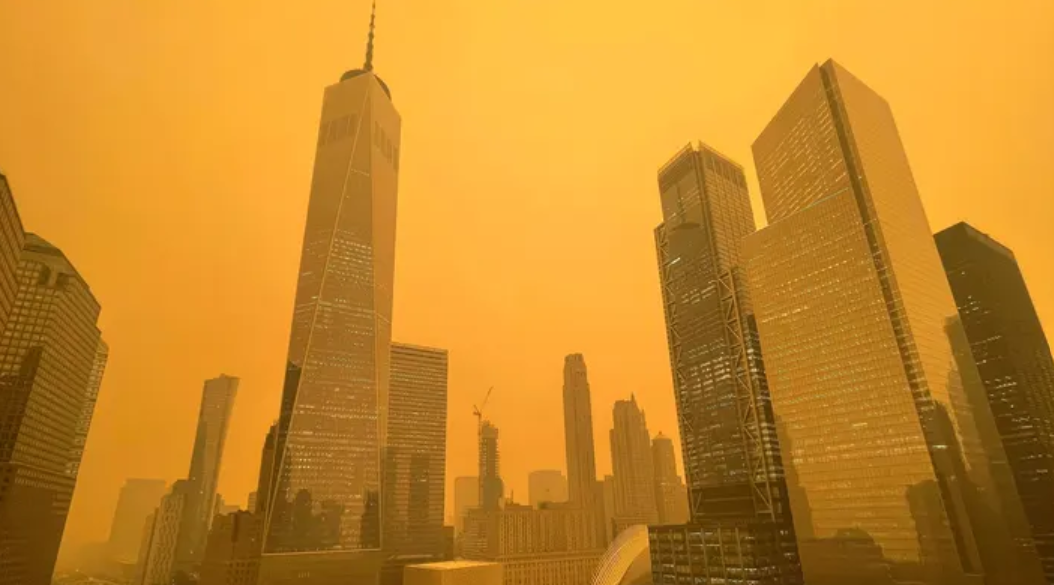
\includegraphics[scale = 0.5]{New York.png}
    \caption{New York during the Canadian wildfire season}
    \label{fig:New York}
\end{figure}
\vspace{0.5 cm}


\subsection{The application of IoT technology}
The Internet of Things refers to the network created by connecting devices embedded with sensors. An Internet of Things system is defined as the set of computationally-capable devices, their sensors and at least one device capable of connecting to the Internet. \par
\vspace{0.5 cm}

IoT devices must not be historically connected devices and not all devices need be connected to the internet, as this would increase the complexity of the system without necessity. An example of such a concept would be found in the still developing \textbf{6LoWPAN} work group of the Internet Engineering Task Force. This work group aims to deliver the capability to use the Internet Protocol to more devices, which may remove the need for edge computers, the devices whose purpose is that of elaborating data and acting as a bridge between sensors and the Internet. \par
\vspace{0.5 cm}
%You could add a paragraph explaining the importance of 6LoWPAN for a system's security, as having a larger surface of attack may lead to undesirable consequences
Regarding the problem of forest fires, an Internet of Things system for both prevention and detection is ideal. Applying this concept we have Dryad\footnote{https://www.dryad.net/}, a private company with the goal of forest health in mind. Their proposed suite shows with excellence what a perfectly engineered IoT system can do for everyone's health and safety. \par
\vspace{0.5 cm}
\newpage
\subsection{Dryad}
Dryad's products offer a service tailor-made for forest health and wildfires. Their suite is composed of 3 different physical devices and their cloud platform.

\begin{itemize}
    \item {\textbf{Wildfire sensor}} A smart sensor capable of sending it's data to the border gateway by using LoRa, either through the mesh gateway or through a single "hop". This device can measure temperature, air humidity and air pressure. It also detects certain gases which, through the help of artificial intelligence, lets it automatically determine if a fire is starting. \par
    \vspace{0.5 cm}
    \begin{figure}[ht]
        \centering
        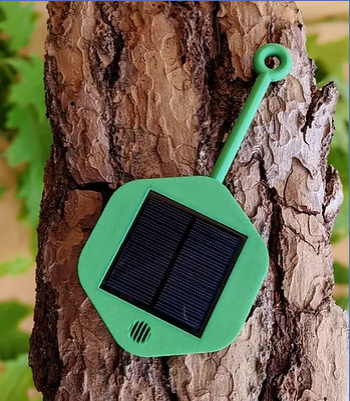
\includegraphics[scale = 0.4]{WildFire Sensor.png}
        \caption{WildFire Sensor}
        \label{fig:WildfireSensor}
    \end{figure}
    \item {\textbf{Mesh gateway}} A device whose main job is that, as the name implies, of creating a mesh grid topology by connecting singular wildfire sensors to itself and connecting itself to other mesh gateways or border gateways.
    They work as extensions to the reach of the border gateway, effectively allowing a far greater reach for the whole system. \par
    \vspace{0.5 cm}
    \begin{figure}[ht]
        \centering
        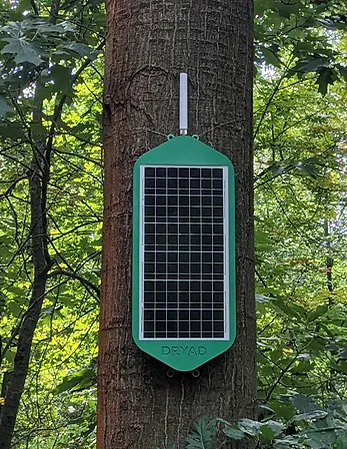
\includegraphics[scale = 0.4]{Mesh Gateway.png}
        \caption{Mesh Gateway}
        \label{fig:Mesh Gateway}
    \end{figure}
    \item {\textbf{Border gateway}} The router of the system. It allows the connection to mesh gateways and wildfire sensors through the LoRaWAN protocol and is connected to the internet through either Ethernet, 4G or satellite up-link \par
    \vspace{0.5 cm}
    \begin{figure}[ht]
        \centering
        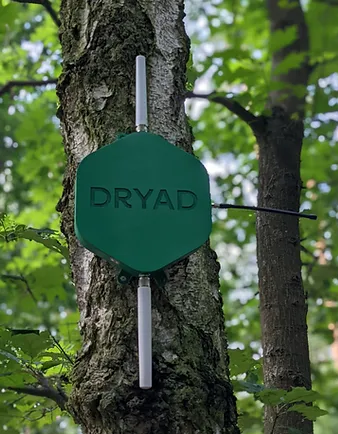
\includegraphics[scale = 0.4]{Border Gateway.png}
        \caption{Border Gateway}
        \label{fig:Border Gateway}
    \end{figure}
\end{itemize}

\newpage

\subsection{The hypothesized system}
Diverging from Dryad's system, the following pages will describe a system that may be used depending on the environment that it is installed in. \par
\vspace{0.5 cm}

Let's start with the definition. An IoT smart box can be defined as the set of sensors and processing units that work together in order to reach a specific and common goal of elaborating the data gathered through the sensors themselves. In addition to Supercaly's definition (See his paper from the sitography) it must be added that a smart box also should include a communication protocol in order to utilize the data without accessing the device directly. \par
\vspace{0.5 cm}

Following Doc. Eng. Romanelli's material handed out in the "Systems for Internet of Things" course, the system shall be described utilizing a bottom-up approach, starting from the sensors all the way up to the connection to the cloud. \par \vspace{0.5 cm}

Moreover, several choices of both hardware and software will be highlighted, finishing the section off with some observations of the system to be implemented.
\section{Architecture and Technology}
\subsection{Sensor Layer}
As mentioned before, the beginning point of any smart box is defined by its sensors. It is essential to capture the nature of the environment we are dealing in. In this case the objective is to monitor the health of the forest soil and the ambient surrounding the box. Thus we can describe the necessary data that the sensors have to provide.\par
\vspace{0.5 cm}
\subsubsection{Data required}
\begin{itemize}
    \item \textbf{Soil moisture:} water is a necessity for forests, much like anything else. In particular soil water is an irreplaceable asset whose presence is mandatory in many Physio-chemical, biochemical and biological processes. Lack of water may also indicate droughts, while excess of water may show problems with the forest's capability to drain rainfall;
    \item \textbf{Air temperature:} trees have a capacity to turn solar energy into water vapour, this process is called "transpiration", as a result the nearby soil is made colder both by being provided shade from the trees and from the process itself;
    \item \textbf{Humidity:} tightly woven together with the need for proper air temperature, forests have an ideal level of moisture to follow. As a plus, both air temperature and moisture can be used to determine the risk level of a forest fire starting in an area; 
    \item \textbf{Air quality:} various gasses may be found in forests. Among these we have pollutants, which worsen the leaves' capacity to photosynthesize. Another crucial factor is the presence of smoke, indicating that a fire might have started.
\end{itemize}
\subsubsection{Sensor options}
Starting with the soil moisture sensors we have our choice split between two categories. \newline
\begin{enumerate}
    \item Resistive moisture sensors: its working principle is based on two probes that let current pass from one to the other, going through whichever medium has the path of least resistance. Measuring the resistance of this circuit will allow to determine the water level of the soil it is installed in. While cheap, easy to use and program, the sensor has a problem due to the probes getting worn down by electrolysis. This makes it unusable for the intended requirements of the project. \newline
    \begin{figure}[ht]
        \centering
        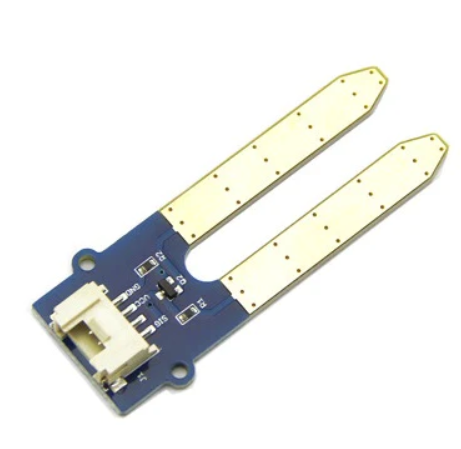
\includegraphics[scale = 0.2]{Resistive moisture sensor.png}
        \caption{Resistive moisture sensor}
        \label{fig:Resistive sensor}
    \end{figure} \newline
    \item Capacitive moisture sensors: a capacitive moisture sensor measures the electrical capacitance between its plates, where changes in capacitance are directly linked to the water content in the surrounding soil due to the differing dielectric constants of air and water. 
    \begin{figure}[ht]
        \centering
        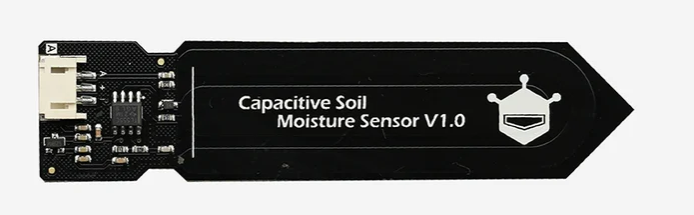
\includegraphics[scale = 0.2]{Capacitive moisture sensor.png}
        \caption{Capacitive moisture sensor}
        \label{fig:Capacitive sensor}
    \end{figure}
\end{enumerate}
\newpage
Following up we have the sensors for air temperature. The cheapest alternatives here are provided by the DHT line of products. 

\begin{figure}[ht]
    \centering
    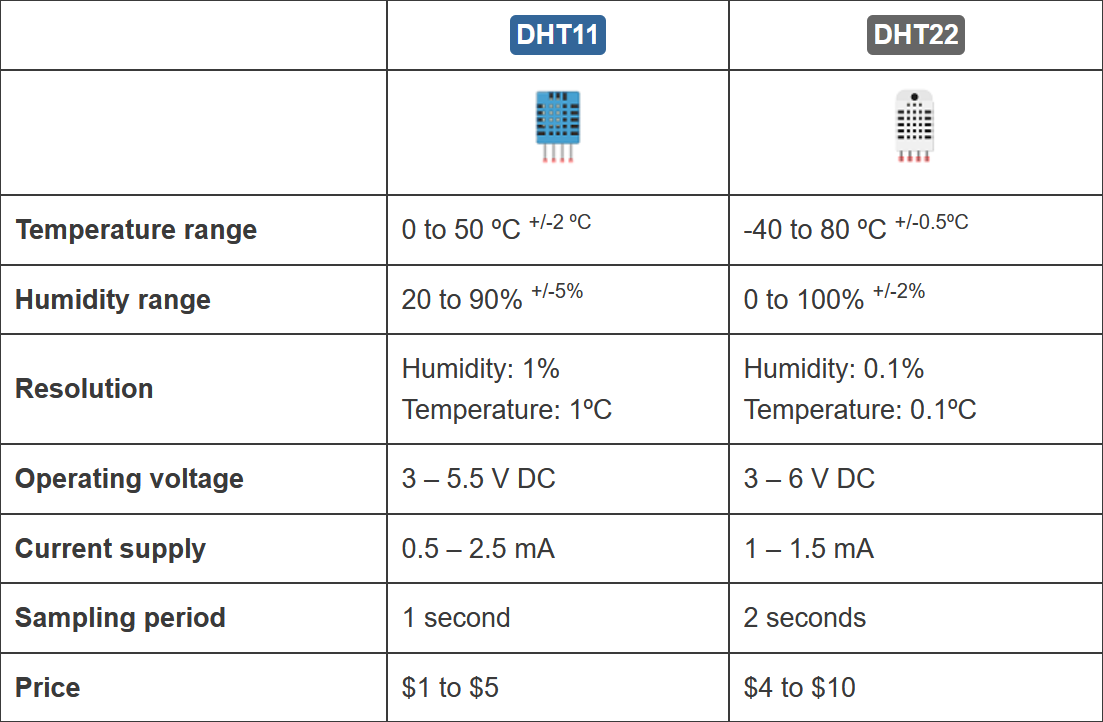
\includegraphics[scale = 0.35]{DHTs.png}
    \caption{Comparison between two types of DHTs}
    \label{fig:DHTComparison}
\end{figure}

From the image above we can decide whichever product is best for our use case. The cheaper option provides us with an ideal price at the cost of worse measurement results. This is actually ideal though, as the sensor's accuracy is beyond our scope, moreover an algorithm could be used in order to calculate the median value of both temperature and humidity, apt to reduce the fundamental inaccuracy of the sensor. \par
\vspace{0.5 cm}
\begin{figure}[h]
    \centering
    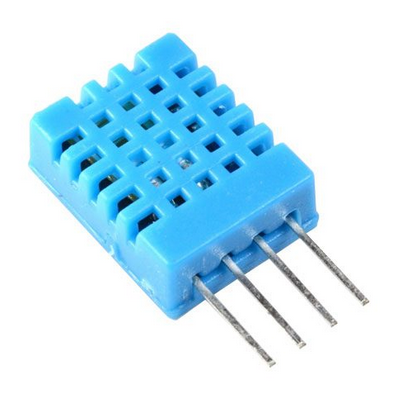
\includegraphics[scale = 0.2]{DHT11.png}
    \caption{DHT11}
    \label{fig:DHT11}
\end{figure}
\begin{figure}[h]
    \centering
    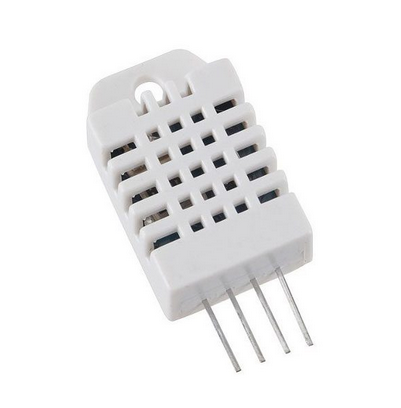
\includegraphics[scale = 0.2]{DHT22.png}
    \caption{DHT22}
    \label{fig:DHT22}
\end{figure}
\vspace{0.5 cm}

Not all use cases will allow for the cheaper option to exalt its abilities. It is enough to mention that most northern regions go very well below 0°C during winter season. On the flip side if a sensor is only being used to determine if a forest fire has started then just about any product of the DHT line will do, even though it would be best to use dedicated hardware. \par
\vspace{0.5 cm}
Air quality is a crucial factor in the detection of forest fires. Mostly dedicated to this purpose, several types can be found, ranging from costing a few euros to even a hundred in the case of smoke detectors. All the main characteristics of the most important sensors are available at this website \url{https://seeeddoc.github.io/How_to_choose_A_Gas_Sensor/} \newline
however for the smart box's function a general purpose, low-cost sensor will suffice. The MQ2 sensor is just right for this endeavor.\par
\vspace{0.5 cm}
\begin{figure}[h]
    \centering
    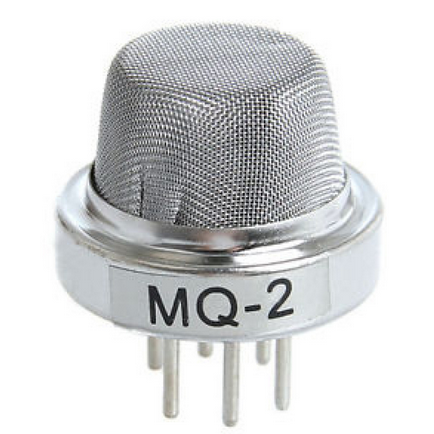
\includegraphics[scale = 0.2]{MQ2.png}
    \caption{MQ2}
    \label{fig:MQ2}
\end{figure}

\subsubsection{Connection to the edge computer}
In any system that relies on sensor data, establishing a reliable connection between the sensors and the processing unit is crucial. This connection ensures that the collected information reaches the processing unit accurately and promptly. In this specific case, where the smart box is self-contained, opting for a wired connection offers several advantages: reliability, cost-effectiveness and simplicity.

\newpage
\subsection{PAN-LAN Layer}
\subsubsection{The Micro-controller}
In order to bind all the aforementioned "dumb" sensors together, a micro-controller is necessary to orchestrate both the out-going and incoming data. An example would be the popular ESP-32 line of products, powerful and versatile micro-controllers that integrate Wi-Fi, Bluetooth, and a dual-core processor on a single chip. The ESP32 products boast a robust set of pins that offer a high degree of flexibility compared to other micro-controllers. Unlike some where specific pins are designated for certain functions, the different ESP32's pins can be configured for various purposes. \par
\vspace{0.5 cm}

\begin{enumerate}
    \item \textbf{ESP32:} Among the ESP32 lineup, the ESP32 stands apart as the pioneering and widely adopted model. It features a potent dual-core Tensilica LX6 microprocessor, along with Wi-Fi and Bluetooth capabilities and a diverse array of peripherals. These attributes render it suitable for a variety of applications, ranging from uncomplicated sensors to intricate IoT devices. Nonetheless, its energy consumption may prove excessive for applications reliant on batteries.
    \begin{figure}[ht]
        \centering
        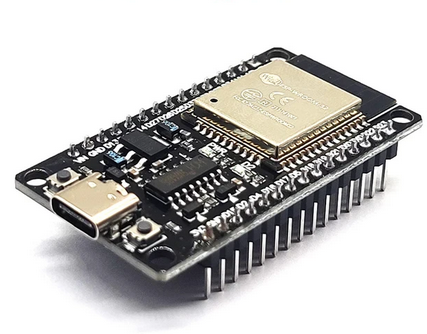
\includegraphics[scale = 0.18]{ESP32.png}
        \caption{ESP32}
        \label{fig:ESP32}
    \end{figure}
    
    \item \textbf{ESP32-C2:} The ESP32-C2 is designed to offer high performance at an affordable price. It has a single RISC-V processor that runs at slower speeds than the ESP32, and it has Wi-Fi and Bluetooth connectivity. However, it has fewer features overall to keep costs down. This makes it ideal for low-cost projects where power consumption is not a major concern.
    \begin{figure}[ht]
        \centering
        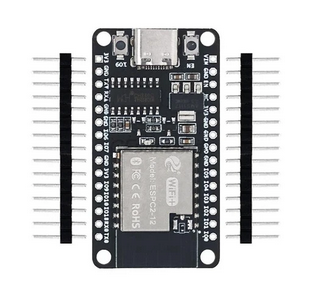
\includegraphics[scale = 0.18]{ESP32-C2.png}
        \caption{ESP32-C2}
        \label{fig:ESP32-C2}
    \end{figure}
    \item \textbf{ESP32-C6:} The ESP32-C6 is the pinnacle of its line, combining a top-notch RISC-V processor with an energy-efficient one. This fusion enables it to handle both power-sensitive tasks and intensive processes. It utilizes the cutting-edge Wi-Fi 6 for lightning-fast and stable connections. Moreover, its support for Thread and Zigbee protocols positions it as a frontrunner for smart home and industrial automation systems.
    \begin{figure}[ht]
        \centering
        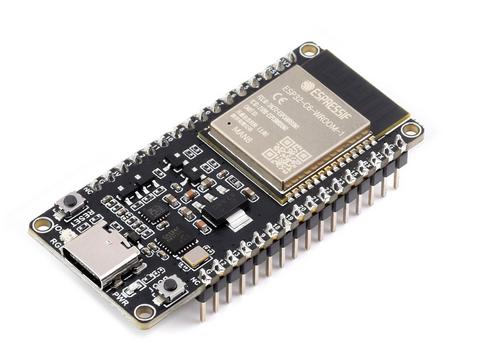
\includegraphics[scale = 0.18]{ESP32-C6.png}
        \caption{ESP32-C6}
        \label{fig:ESP32-C6}
    \end{figure}
    \item \textbf{ESP32-H2:} The ESP32-H2 is a power-efficient micro-controller that aims to extend battery life in IoT devices. It has a single RISC-V processor with power-saving features. It supports Thread and Zigbee protocols, enabling low-power mesh networking in IoT applications, making it suitable for battery-operated devices that need to run for extended periods of time.
    \begin{figure}[ht]
        \centering
        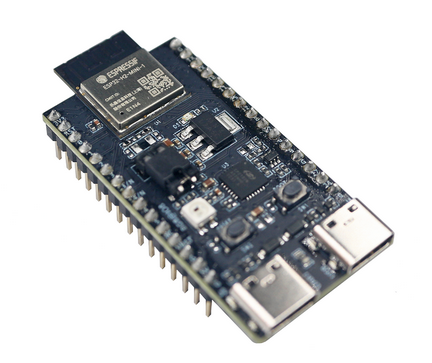
\includegraphics[scale = 0.18]{ESP32-H2.png}
        \caption{ESP32-H2}
        \label{fig:ESP32-H2}
    \end{figure}
\end{enumerate}

\subsubsection{The energy supply}
The necessity to have some type of energy supply comes from the longevity requirements set by our use-case standards. This is the reason as to why a supply system composed of strictly energy accumulators is not recommended. \par
\vspace{0.5 cm}

Solar panels are the answer for this. Much like calculators these are the only device that would allow the smart box to gather energy while also being installed on the box itself. \par
\vspace{0.5 cm}

Not much research was found proposing the idea of a fully self sustaining forestry smart box, thus some experimentation would be in order. Let's break down some essential considerations:
\begin{itemize}
    \item \textbf{Low maintenance:} solar panels benefit from low maintenance: the only real cost would be cleaning them when their efficiency gets too low.
    \item \textbf{Adverse weather conditions:} solar energy harvested by solar panels is heavily dependant on weather conditions. This unreliability means that whole grids could shut off based on geographical location and season, or even if the required power supply is greater than what the solar panel can provide.
    \item \textbf{Power savings mode:} while hosting a wide range of features to reduce power consumption (see ESP32's Deep Sleep) these cannot be used due to them turning off most peripherals, including the wireless connectivity, whether this be Wi-Fi, Thread, ZigBee or BLE. This is an unacceptable option as it wouldn't allow for smart boxes to act as a system.
    \item \textbf{Increasing the system size:} this is dependant on the used communication protocol. It both depends on which protocol is used and the amount of data transferred. We can deduce then that higher data traffic means more node usage, which in turn means higher power consumption.
    \item \textbf{Clock gating:} one of the most popular options in power saving technology is allowing the clock-gating of the CPU. Indeed by reducing the max speed of the micro-controller the longevity of the system would increase at the cost of a possible slow-down of the throughput of information.
\end{itemize}


\subsubsection{The energy accumulator}
Despite the low power usage, smart boxes must have the ability to keep going without maintenance for long periods of time. The provided use case proves this by requiring to be almost completely autonomous. It is indeed unthinkable to require maintenance on smart boxes that are dug in the middle of a massive forest. \par
\vspace{0.5 cm}

To this effect capacitors could be used to power the system, an ideal component that is small, durable, field-tested and cheap. However their main flaw resides in their lack of energy density, meaning an assured incapability to sustain the smart box in periods where energy isn't being gathered. \par 
\vspace{0.5 cm}

This would require testing, especially as the smart box network increases it would mean a not necessarily linear energy discharge and since Dryad's system denotes the strict usage of capacitors for their sensors. A backup option is thus found in batteries. \par
\vspace{0.5 cm}

Traditional batteries, whichever the form, are a secondary but most likely mandatory plan. These would allow for the device to work during periods in which energy isn't being accumulated in the capacitors. A backup that could very well be a point of failure as batteries aren't renowned for their longevity. For now, however, they remain one of the options.\par
\vspace{0.5 cm}

\subsection{Communication protocol from edge computers to the router}

As previously defined each smart box will host its own micro controller, capable of wireless transmission of data. Referring to the ISO/OSI stack we determine two different paths to reach the desired goal of connecting every smart box to the router. In each case a mesh topology is desirable as it allows for unprecedented reach. \par 
\vspace{0.5 cm}

The main divergence from the system proposed by Dryad can be found in the smart box being able to connect itself to similar boxes that host the same communication protocols. The next section will talk about the proposed protocols, highlighting the pros and cons. \par
\vspace{0.5 cm}

\subsubsection{ESP-MESH}

Climbing the OSI stack we find a protocol destined for use by Espressif's ESP32 line of products: ESP-MESH. \par \vspace{0.5 cm}
ESP Mesh networking is a line of libraries dedicated to defining the protocols and APIs necessary to allow communication of ESP devices. These libraries are split into two categories:
ESP-WIFI-MESH and ESP-BLE-MESH. \par \vspace{0.5 cm}

Starting off with ESP-WIFI-MESH, we have a networking protocol built utilizing the Wi-Fi protocol. ESP-WIFI-MESH enables the connection of many devices spread over a large physical area into a single Wireless Local-Area Network. \par \vspace{0.5 cm}

ESP-WIFI-MESH Also boasts the capacity to self-organize and self-heal, effectively allowing autonomous building and maintenance. The protocol's most pertinent quirks will therefore be pointed out and described, while the rest can be read in Espressif's website for ESP APIs \par \vspace{0.5 cm}
\begin{itemize}
    \item \textbf{A different approach to connectivity:} a traditional Wi-Fi network is a point-to-multipoint network where the central node is denoted as "access point" and represents the WAN-Enabled device that permits the connection to the internet. \par \vspace{0.2 cm}
    ESP-WIFI-MESH changes this by allowing each node\footnote{In this case a node represents a smart box} of the system to connect to neighbouring nodes. One potential, fatal flaw is the increase in points-of-failure, as nodes will require other nodes in order to reach connection. Such a flaw is easily fixed by allowing a node to connect to multiple other nodes, bringing the network to have unrivaled resilience. \par \vspace{0.2 cm}
    \item \textbf{Node Typing:} ESP-WIFI-MESH differentiates each node and gives each class its own job. Four types of nodes are found in a ESP-WIFI-MESH network, necessarily starting with the first node, the Root Node. \par \vspace{0.2 cm}\textbf{The Root Node} acts as the interface between the router (WAN Connection) and the ESP-WIFI-MESH network. Only one root node is allowed per network, this doesn't cause an issue with points of failure though as the network allows for both manual and automatic root node selection, thus providing a backup if the root node fails.  \par \vspace{0.2 cm}
    \textbf{Leaf Nodes} are nodes that either don't satisfy the softAP interface (this means that other nodes cannot connect to it) or that have reached the last layer of nodes, which is a setting for the network itself. These nodes act as transmitters but not receivers, thus they cannot relay other nodes' packets. \par \vspace{0.2 cm}
    \textbf{Intermediate Parent Nodes} are nodes that act as transceivers. Both capable of receiving and sending data, but also capable of connecting other nodes through their softAP interface. \par \vspace{0.2 cm}
    \textbf{Idle Nodes} are nodes that haven't connected to the network, these can either connect to an intermediate parent node or become a root node, if the settings of the network allow it. \par \vspace{0.2 cm}
    \item \textbf{Data Transmission:} being built on top of the Wi-Fi protocol, ESP-MESH packets are composed of the header, split into source address, destination address and options, and the payload itself. The payload could be binary code or could be encoded under an application layer protocol. 
\end{itemize}

ESP-BLE-MESH Is also available and it works on the specifications defined in IEEE's 802.15.1 But will not be covered.

\subsubsection{The 802.15.4 Physical and Medium Access Control layer}

The 802.15.4 Physical Layer offers low-cost, low-speed communication between devices. It is a wireless communication protocol capable of 10 meters of communication range with a transfer rate of 250 kbit/s. Lower power requirements are reachable through the reduction of the transfer rates. \par
\vspace{0.5 cm}

Notable features for this layer are:
\begin{itemize}
    \item Support for secure communications
    \item Power management functions
    \item Three working frequency bands: 865/915/2450 MHz
\end{itemize}

Given the chosen environment for the smart box, the lower-end of the radio frequency spectrum allows for less interference and more object penetration, a critical factor due to the abundant presence of water in most organic matter. \par
\vspace{0.5 cm}

The physical layer of 802.15.4 provides the communication of devices through radio transceivers (transmitter and receiver), allowing for channel hopping in order to reduce interference. This layer works on the aforementioned unlicensed frequency bands. 
\par
\vspace{0.5 cm}

As for the MAC layer, the protocol allows for unfragmented frames to be shared through the physical channel.

\subsubsection{6LoWPAN}

6LoWPAN is an IPv6-based protocol apt to bring IP connectivity to the smallest devices, allowing them to participate in the proposed IoT system. It can work on various different protocols. 
\par
\vspace{0.5 cm}

\subsubsection{Thread}

Thread is a low-power mesh networking technology based on IPv6. Thread uses 6LoWPAN, which in turn uses the 802.15.4 MAC and PHY layers. The selected working frequency band is in the 2.4 GHz spectrum. \par \vspace{0.5 cm}

Thread uses connecting routers (necessary for the 6LoWPAN architecture) with the name of "Border Routers", allows for the mesh network to self-heal and doesn't have a single point of failure, by architecture's standards. 

\subsubsection{LoRa Physical layer}
LoRa (Long Range) technology was developed by a french company called Cycleo, then acquired by Semtech. The modulation scheme is based on the "Chirp Spread Spectrum" spectrum spreading technology. \par \vspace{0.5 cm}

This spreading technology uses a selectable radio parameter called Spreading Factor, which ranges from 5 to 12. This factor represents the number of bits sent per symbol, where a symbol is represented by a cyclic shifted chirp. This effectively means that a low spreading factor yields a higher data rate but worse sensitivity, and vice versa. \par \vspace{0.5 cm}

Despite the higher error tolerance, a lower spreading factor also means a longer time for the modem to be transmitting data, which in turn leads to consuming more energy. Pre-existing studies of LoRa performances already exist and could be utilized in order to have an ideal trade-off of data rate, error sensitivity and power usage. \par \vspace{0.5 cm}

Lora operates in the unlicensed ISM bands, at 868 MHz in Europe, with other frequencies in the Americas, India and Asia. \par \vspace{0.5 cm}

\subsubsection{LoRaWAN MAC layer}

LoRaWAN is the MAC layer protocol based off of the LoRa physical layer, upon which it provides long range, low-power communication. LoRaWAN manages communication frequencies, data rate and power for the devices, which transmit data whenever available. \par \vspace{0.5 cm}

The data is gathered by LoRaWAN gateways, responsible for delivering the data to the central network, effectively creating a "star of stars" topology. \par \vspace{0.5 cm} 

\subsubsection{Unofficial LoRa Meshing Libraries}
Instead of using LoRaWAN, whose architecture requires the use of gateways, the focus could be brought onto the devices themselves. Changing the topology from a "star of stars" to a mesh network would allow for each smart box to be strongly connected to the rest of the system, allowing for a robust grid of communication that is a perfect fit for the given use case. \par \vspace{0.5 cm}

One example is LoRa MESH, an ad-hoc network communication protocol. It offers both LoRa's technological advantages and the benefits of a mesh network. Using this protocol we can expect the network to be self-organizing, self-healing and to be highly flexible and scalable. \par \vspace{0.5 cm}

The architecture is divided into two types of nodes, the routing node is able to receive data for routing updates and data forwarding. Meanwhile the terminal node doesn't have routing functions and are deployed in the edges of the network. \par \vspace{0.5 cm}

As typical of a mesh network, multi-hop transmission is granted between router nodes, while the low power requirements of LoRa grant that each transmitted package will have little impact on the power usage of the intermediate nodes. \par \vspace{0.5 cm}

LoRa MESH allows for four different communication methods: 
\begin{enumerate}
    \item Unicast: a one-to-one message, ideal to send messages to the terminal nodes or the nodes connected to external networks;
    \item Broadcast: an unrestricted one-to-many message;
    \item Multicast: a restricted one-to-many message, possibly useful if multiple routers are present on the network, but hard to implement;
    \item Anycast: can either use unicast and broadcast, but regardless it usually sends a message to the "best" node.
\end{enumerate}

Finally, LoRa MESH has unlimited routing during broadcast communication and can form massive networks. The theoretical maximum of nodes allowed in a network is 65535. \par \vspace{0.5 cm}

\subsection{WAN Layer}
\subsubsection{The router}
In the WAN Layer we find the devices whose goal is that of connecting the entirety of the LAN and sensor layers to an external network, usually the Internet. For this purpose we have a critical choice between dividing components or having one "do it all" piece of hardware. \par \vspace{0.5 cm}

On one hand the components can be divided: this means that a fully-fledged router, including its OS, can be utilized. Most routers include both Wi-Fi and Ethernet LAN as per 802.11 standards however other types of connectivity are scarcely available, such as the suggested 802.15.4 or LoRa, this means that at least one node should act as an intermediary, being able to connect from the router to the rest of the network. \par \vspace{0.5 cm}

\begin{figure}[ht]
    \centering
    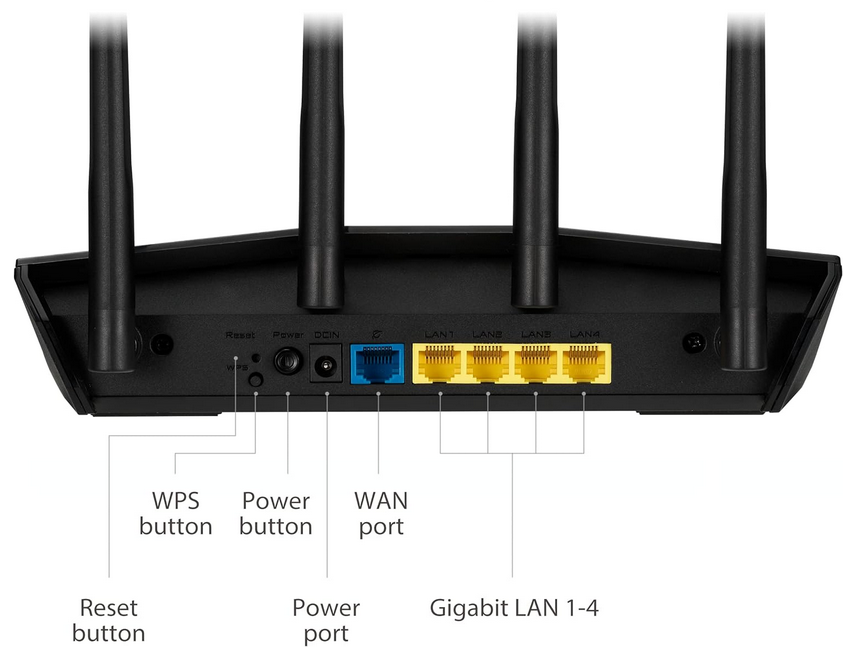
\includegraphics[scale = 0.2]{Asus RT-AX1800S Ports.png}
    \caption{The ports offered by the Asus RT-AX1800S router}
    \label{fig:Asus RT-AX1800S Ports}
\end{figure}

Given the amount of data to be sent over LoRa to the intermediary, a standard Wi-Fi connection to the router should suffice. Wi-Fi connectivity is granted by most ESP32 boards and external modules that allow Ethernet connection are also available commercially.\par \vspace{0.5 cm}


On the other hand, one singular device could be used to guarantee WAN and LAN connectivity. One such example is found in the ESP32-SIM7600 board. 
\begin{figure}[ht]
    \centering
    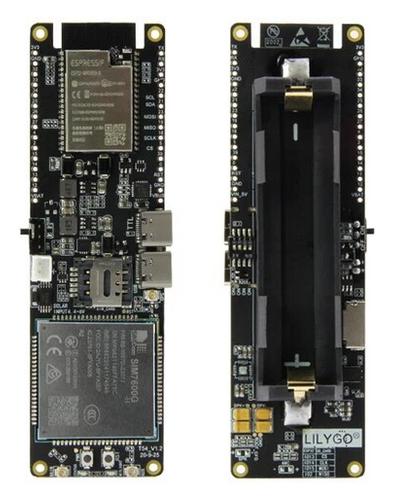
\includegraphics[scale = 0.2]{ESP32 SIM7600.png}
    \caption{ESP32 SIM7600}
    \label{fig:ESP32 SIM7600}
\end{figure}

As can be seen in the technical documentation, this SoC has an already integrated battery (model 18650) shield and solar panel pins, while also including a sim slot for 2G/3G/4G connectivity. 

\subsubsection{Communication protocol from router to Internet}
As mentioned above, communication with the Internet must be established for the system to work correctly. Two choices were thereafter given, one including the possibility of relaying the networking job to a fully fledged router, so to delegate the data link and physical connectivity to a device not too different from the rest of the network. The other being a node with the same connectivity as well as access to Internet \par \vspace{0.5 cm}

Considering the low amount of router cells necessary in the system, reliability is a greater factor than the price, thus a router sounds like the best option. In such a case most routers own an operative system that is well capable and structured to guide your hand to connecting your network to the internet. Among such options, we have port forwarding which allows the direct access to a specific server of a network. \par \vspace{0.5 cm}

Picking up the ESP32 SIM7600 instead, a sim card is used to connect your smart box; however, this comes at the price of having an unprogrammed device to deal with and less flexibility, with features like firewalls being absent. Moreover, cellular data plans may incur charges based on the amount of data being transferred. Unlimited data \textbf{upload} is ideal considering the use case.
\subsection{Cloud Layer}

Finally, having reached the cloud layer, only the communication protocol to the WAN remains to be defined, as the data that is gathered by the network must be available 24/7. For this, it is enough to mention the use of the HTTP protocol. \par \vspace{0.5 cm}

The HTTP, or Hypertext Transfer Protocol, is the basis for communication on the Internet. It outlines how information is shared between web browsers and servers. It follows a request-response setup, where a browser asks for a particular resource (such as a web-page) by sending a request to the server. The server then handles the request, gets the resource, and replies with a response that includes the data and other details. This interaction lets users engage with web content, get files, and find info online.\par \vspace{0.5 cm}

At the cloud layer, the geographical location of devices loses meaning, allowing users to benefit from services hosted by computers in unknown areas of the world. Your data may very well be in a Roman data center or be held in multiple, split servers in both Mexico and Japan. Below are some definitions that better explain the cloud layer and the services offered by it. \par \vspace{0.5 cm}

The cloud layer, or rather cloud computing, is a type of business model that aims to virtualize computer resources and offer them as a service in its different aspects. This service is to be either paid for or free, and can be found under many facets. Services may differ from storing space for their users (such as in the example above) to streaming videos (Youtube, for example). The cloud layer is divided into services, as below. \par \vspace{0.5 cm}

\begin{figure}[ht]
    \centering
    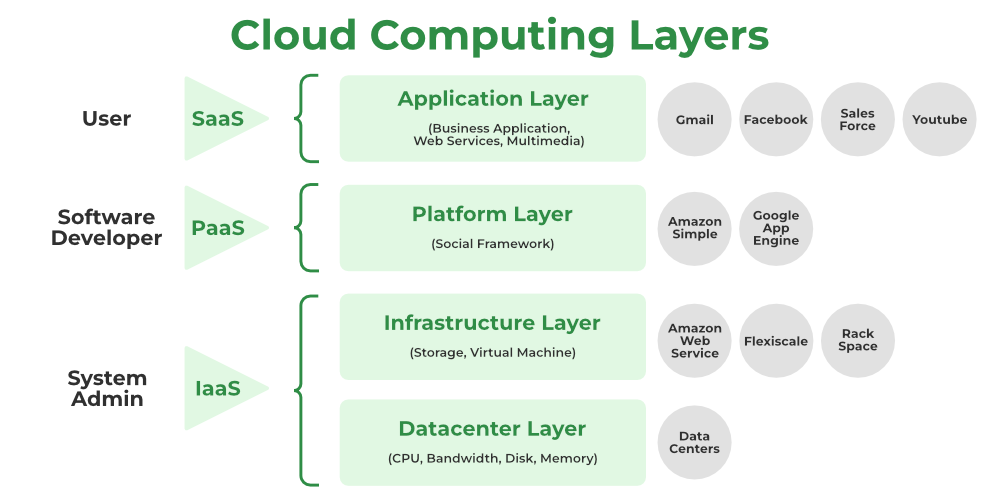
\includegraphics[scale = 0.4]{Cloud Computing Layers.png}
    \caption{Cloud Computing Layers}
    \label{fig:Cloud Computing Layers}
\end{figure}

\begin{itemize}
    \item \textbf{Infrastructure as a Service:} this layer has hardware resources, usually resources are allocated on demand or when a platform requires them.
    \item \textbf{Platform as a Service:} this layer hosts platforms instead of single programs. 
    \item \textbf{Software as a Service:} this last layer sits atop the other ones and presents singular programs that already benefit from the layers below, concealing the inner workings to the user. 
\end{itemize}

\par \vspace{0.5 cm}

Having mentioned such definitions, we now shift our focus to the project at hand. Surveillance tasks such as the ones that smart boxes allow us to require to be accessible at all times and alert qualified personnel whenever needed. \par \vspace{0.5 cm}

Cloud computing offers services tailored for this. Hosting a web server and storing the gathered data using the cloud is simple enough and could prove to be cheaper than using private resources in order to reach this goal. An alternative would be to use the ESP32 destined as the master, or root node, to work as a web server, opening its HTTPS port (443) and broadcasting the necessary data to the Internet. At the same time it could send data through the internet and onto remote storage or save it locally, requiring large data banks to be installed on-site. Another downside of local storage is found in its scalability. \par \vspace{0.5 cm}

If automatic fire detection is required, artificial intelligence could be used to study the data and give accurate predictions of where and when fires could occur. The main issue with artificial intelligence lies in the large databases it has to train on in order to be the most accurate possible and the computational resources that it uses. This would make it really difficult to host such an algorithm in a distributed matter, that is to allow each smart box to utilize the algorithm. Such a task would also kill the battery hosted by each smart box, effectively disabling the network in the worst-case scenario. With such a problem at hand a simple solution is once again found in cloud computing. \par \vspace{0.5 cm}

\section{Cyber Security}

\subsection{Definitions}
The Internet of Things (IoT) has rapidly grown, ushering in a new era of innovation and convenience alongside fresh security concerns. As more devices link to the internet, ranging from smart home gadgets to industrial sensors, safeguarding these interconnected systems becomes essential. The protection of data collected and sent by these devices plays a critical role in maintaining privacy, avoiding operational hiccups, and promoting the wellbeing of the IoT network. \par \vspace{0.5 cm}

In our case, the main concern lies within the connection from and to the cloud. Encryption is the method of defence with which this project is concerned. As IoT devices struggle with encryption due to the computational and energy usage limitations. Thus we define the attack surface as follows: \par 

\begin{quote}
    The attack surface of a software environment is the sum of the different points (for "attack vectors") where an unauthorized user (the "attacker") can try to enter data to, extract data, control a device or critical software in an environment. Keeping the attack surface as small as possible is a basic security measure.
\end{quote} from Wikipedia. \par \vspace{0.5 cm}

Now knowing what is being protected, we will follow up by listing the types of encryption hosted by the different communication protocols, and some types of attacks that would exploit the vulnerabilities of the system.

\newpage

\subsection{Sensor Layer}
As already mentioned, every sensor's data is immediately sent to the microcontroller through a wired connection. The problem with this is that if no precautions are taken, it makes it really easy to override such data; effectively feeding false information about the grid. This may result in false detection of fires, such as if the humidity sensor signals the lack of humidity or if the MQ-2 sensor is compromised to show an erroneous presence of CO2 in the area. This very well may be abused by ill-intentioned people to show a presence of fires that isn't actually there in order to reach a certain goal. This type of attack would fall into the "poisoning" category, in which data is tampered with by a third party. Whether this be intentional or accidental an ideal defense has several options to choose from.
\par \vspace{0.5 cm}

Options to defend against poisoning or data would include pre-existing methods, such as the one used by processors to avoid showing what instructions are being used: these devices indeed can detect when the power supply's wires have been cut, thus shutting off activity when dealing with an unauthorized power supply. In the same way the chosen processor may be adapted to shut off sensor communication whenever a cut in the feed is detected. \par \vspace{0.5 cm}

Other types of attacks may include direct tampering with the sensors, such as holding a lighter next to the temperature sensor. While this situation may prove difficult to intervene in, the easiest solution would be to train the machine learning algorithm to detect such harsh changes in values, however this may reduce performance or accuracy in the system. \par \vspace{0.5 cm}

Finally, a worthwhile mention is that the showcased sensors do not have the capacity to encrypt data, allowing third parties to read such data without issue. However this would likely prove to be far too laborious work to justify overriding thousands of sensors. Putting this under the scope of national security, if an opponent nation required to spy the nation's forests looking for fires it would be faster and less intrusive to simply use pre-existing tech, such as satellite imaging or UAV reconnaissance \par \vspace{0.5 cm}  

\newpage

\subsection{PAN-LAN Layer}

In the PAN and LAN layers we found vulnerabilities in the connection between the various microcontrollers and, if used, the router. All the chosen communication standards are wireless and as such, prone to being sniffed, redirected or even blocked. Physical means of interfering with the communication of the grid is as simple as creating a Faraday cage around the object to isolate, while sniffing may be done through an antenna that communicates within the same band of frequencies of the system. A type of redirection is found in MITM attacks. This could be done in various ways, more notably through MAC spoofing or IP spoofing; these are easily accessible technologies and prove dangerous if an AAA system isn't implemented. \par \vspace{0.5 cm}

Starting from the definition of MITM attack: \begin{quote}
    In cryptography and computer security, a man-in-the-middle (MITM) attack, or on-path attack, is a cyberattack where the attacker secretly relays and possibly alters the communications between two parties who believe that they are directly communicating with each other, as the attacker has inserted themselves between the two parties.
\end{quote} from Wikipedia \par \vspace{0.5 cm}

and continuing with the definition of AAA Protocol: \begin{quote}
    AAA refers to Authentication (to prove identity), Authorization (to give permission) and Accounting (to log an audit trail).
    It is a framework used to control and track access within a computer network. 
\end{quote} from Wikipedia \par \vspace{0.5 cm}

As the site informs us, an effective way to reduce the possibility of a MITM attack is through the AAA protocol; or more exclusively the authentication and authorization parts of the protocol. Considering that the proposed system uses a fixed-size computer network a simple way of authenticating AND authorizing would be to have a AAA server allowing devices to connect to the grid and only have clearance to send data to the router once logged in. As for accounting it is quite straightforward as authentication implies that each node has a different identity which allows for individual logging of data. \par \vspace{0.5 cm}

Finally, in order to rule out sniffing it is enough to utilize communication protocols that use encryption to protect their data. 
Following up is each aforementioned standard's (See "Communication protocol from edge computers to the router") encryption capability. 
\begin{itemize}
    \item [802.11]
    The 802.11 protocol has different encryption protocols available, among these we find: WEP, WPA, WPA2 and WPA3, in increasing order of complexity to decode. Do note that WPA2 uses AES encryption.
    \begin{itemize}
        \item ESP-WIFI-MESH
        \item ESP-BLE-MESH
    \end{itemize}
    \item [802.15.4]
    The 802.15.4 protocol uses the AES with a key length of 128 bit, that is 16 bytes. It is used by the following protocols
    \begin{itemize}
        \item 6LoWPAN
        \item Thread
    \end{itemize}
    \item [LoRaWAN and Mesh]
    The LoRaWAN and Mesh protocols also use AES encryption
\end{itemize}

It is then easy to see that most protocols use AES encryption, below is the definition:
\begin{quote}
    The Advanced Encryption Standard (AES), also known by its original name Rijndael, is a specification for the encryption of electronic data established by the U.S. National Institute of Standards and Technology (NIST) in 2001.
\end{quote} from Wikipedia

AES encryption is in fact so good that we cannot expect it to keep working uncracked, indeed plenty of holes have already been opened up in its algorithm, leading to decreased cracking times than regular brute force attempts. For how reassuring this may sound however, AES allows for longer key sizes, such as 192, 256, 512 or 1028 bits; this makes it so that brute force attempts take longer at the cost of increased encryption computation requirements. \par \vspace{0.5 cm}

Finishing off with sniffing and encryption in general, it is mandatory to guarantee the proper encryption of data before it is transmitted. The problem with such a statement is that microprocessors struggle with the computational requirements of such high level encryption algorithms. \par \vspace{0.5 cm}

\subsection{WAN Layer}

Some introductory definitions are needed:

\begin{quote}
    Transport Layer Security (TLS) is a cryptographic protocol designed to provide communications security over a computer network. The protocol is widely used in applications such as email, instant messaging, and voice over IP, but its use in securing HTTPS remains the most publicly visible. 
\end{quote} from Wikipedia \par \vspace{0.5 cm}

\begin{quote}
    The Transmission Control Protocol (TCP) is one of the main protocols of the Internet protocol suite. It originated in the initial network implementation in which it complemented the Internet Protocol (IP). Therefore, the entire suite is commonly referred to as TCP/IP. TCP provides reliable, ordered, and error-checked delivery of a stream of octets (bytes) between applications running on hosts communicating via an IP network. Major internet applications such as the World Wide Web, email, remote administration, and file transfer rely on TCP, which is part of the Transport layer of the TCP/IP suite. SSL/TLS often runs on top of TCP. 
\end{quote} from Wikipedia \par \vspace{0.5 cm}

Now talking about the WAN Layer, it can be taken for granted that the ruling standard is TCP/IP, that is a connection that uses the TCP transport layer with the IP networking layer. In the WAN Layer we find that our IP packet will most likely be endangered if not encrypted, to this effect TLS provides an efficacious method of encryption that simply requires us to specify both an IP and the port being used; usually the port is 443. \par \vspace{0.5 cm}

\newpage

\section{Conclusion}

In conclusion we find that plenty of secure methods are available for use, with the main challenge being energy accumulation. Similar systems may be used in other use cases, such as Smart City car parking and such. In this case the main focus is long-range, stable and low power connectivity, thus LoRa + LoRaWAN/Mesh should be used in order to establish secure communication, possibly using ESP-MESH for creating clusters of nodes in order to increase the coverage of the sensors in the area. As for WAN connectivity a router should be capable enough to deal with all the data, sending it to a secure web server through TLS whose job is displaying the gathered data and, if necessary, be able to send a mail to local authorities if a connected machine learning algorithm detects a fire. 

\section{Sitography}
\begin{itemize}
    \item \url{https://www.nature.com/articles/d41586-023-04033-y}
    \item \url{https://phys.org/news/2023-06-canada-co2-emissions-year.html#:~:text=Worldwide%2C%20wildfires%20in%202021%20released,from%20fossil%20fuels%20and%20industry.}
    \item \url{https://psiborg.in/forest-fire-detection-using-sensor-network-and-iot/}
    \item \url{https://www.dryad.net/}
    \item \url{https://github.com/Supercaly/esame-internet-of-things}
    \item \url{https://www.intechopen.com/chapters/72698}
    \item \url{https://www.vulhm.cz/en/forests-control-soil-moisture-and-air-humidity/}
    \item \url{https://store.arduino.cc/products/grove-moisture-sensor?queryID=undefined}
    \item \url{https://store.arduino.cc/products/gravity-analog-capacitive-soil-moisture-sensor-corrosion-resistant}
    \item \url{https://www.canadarobotix.com/blogs/how-to/soil-moisture-sensor-resistance}
    \item \url{https://randomnerdtutorials.com/esp32-dht11-dht22-temperature-humidity-sensor-arduino-ide/}
    \item \url{https://www.oneearth.org/ecoregions/mid-canada-boreal-plains-forests/}
    \item \url{https://seeeddoc.github.io/How_to_choose_A_Gas_Sensor/}
    \item \url{https://en.wikipedia.org/wiki/IEEE_802.15.4}
    \item \url{https://en.wikipedia.org/wiki/6LoWPAN}
    \item \url{https://en.wikipedia.org/wiki/Thread_(network_protocol)}
    \item \url{https://docs.espressif.com/projects/esp-idf/en/stable/esp32/get-started/index.html}
    \item \url{https://en.wikipedia.org/wiki/LoRa}
    \item \url{https://hal.science/hal-01977497/document}
    \item \url{https://www.cdebyte.com/news/587#a6}
    \item \url{https://hackaday.io/project/188566-devkit-esp32s3-sim7600}
    \item \url{http://www.airspayce.com/mikem/arduino/RadioHead/}
    \item \url{https://en.wikipedia.org/wiki/Cloud_computing}
    \item \url{https://en.wikipedia.org/wiki/Attack_surface}
    \item \url{https://en.wikipedia.org/wiki/Spoofing_attack}
    \item \url{https://en.wikipedia.org/wiki/Man-in-the-middle_attack}
    \item \url{https://en.wikipedia.org/wiki/AAA_(computer_security)}
    \item \url{https://en.wikipedia.org/wiki/Advanced_Encryption_Standard}
    \item \url{https://en.wikipedia.org/wiki/Transmission_Control_Protocol}
    \item \url{https://en.wikipedia.org/wiki/Transport_Layer_Security}
\end{itemize}






\end{document}